\chapter[ADNEX VS RMI]{Head-to-head comparison of the RMI and ADNEX models to estimate the risk of ovarian malignancy}
% Only include if the thesis is written as a collection of papers
%_________________________
\includegraphics*[width=0.4\linewidth]{logos/BMJ_Open.png}
\label{sec:chp_ADNEXvsRMI}

\glsunset{ADNEX}
\glsunset{AUC}
\glsunset{CHARMS}
\glsunset{CI}
\glsunset{CrI}
\glsunset{GRADE}
\glsunset{IOTA}
\glsunset{JAGS}
\glsunset{NB}
\glsunset{OSF}
\glsunset{PI}
\glsunset{PRISMA}
\glsunset{PROBAST}
\glsunset{PROSPERO}
\glsunset{RMI}
\glsunset{ROC}
\glsunset{RU}
\glsunset{TRIPOD}
\vspace{0.5cm}

published as: 
\begin{quote}
 \textbf{Barreñada L}, Ledger A, Kotlarz A et al. Head-to-head comparison of the RMI and ADNEX models to estimate the risk of ovarian malignancy: a systematic review and meta-analysis of external validation studies. \textit{BMJ Open}. 2025;15:e104141. \url{https://doi.org/10.1136/bmjopen-2025-104141}
\end{quote}
\begin{quote}
 \textbf{Supplementary material and code} available in the online version and at \url{https://osf.io/nt89z/}.
\end{quote}


\vspace{-0.5em}
\noindent\scriptsize\textit{Submitted: 23/04/2025 \quad Published: 04/08/2025 \quad (103 days) \quad APC: 2390 \pounds}
\normalsize\vspace{-0.5em}

\section*{Summary}
We extended the systematic review and meta-analysis of external validations of the \gls{ADNEX} model
 (Chapter \ref{sec:chp_ADNEXSR}) to perform a head-to-head comparison of the performance of the \gls{ADNEX} and \gls{RMI} models. We included 11 studies with 8271 tumours. The performance of \gls{ADNEX} was better than that of \gls{RMI} in terms of discrimination and clinical utility. The probability of the model being useful in a hypothetical new centre in operated patients was 96\% for \gls{ADNEX} with CA125 and 15\% for \gls{RMI} at the 10\%  threshold. The results support the use of \gls{ADNEX} instead of \gls{RMI} for triaging patients with ovarian tumours for referral to an oncology centre.

\newpage

\section{Introduction}

To choose the optimal management of an ovarian mass, the characterisation of the
mass as benign or malignant is essential to improve treatment outcomes
 \cite{timmermanESGOISUOGIOTA2021,ledermannESGOESMOESP2024}.
If the mass is likely to be malignant, treatment in a referral centre for
gynaecological oncology improves the outcome
 \cite{harterImpactStructuredQuality2011,alettiQualityImprovementSurgical2009}.
The Assessment of Different NEoplasias in the adneXa (\gls{ADNEX}) model
 \cite{vancalsterEvaluatingRiskOvarian2014} and the Risk of Malignancy Index (\gls{RMI})
 \cite{jacobsRiskMalignancyIndex1990} have become key tools for estimating the risk
of an ovarian mass being malignant.

\gls{RMI} provides a non-negative value that is associated with malignancy
 \cite{jacobsRiskMalignancyIndex1990}. A commonly used cut-off to classify a tumour
as high risk for malignancy is 200
 \cite{OvarianMassesPremenopausal2016a,AggstockscancerMedEpitelial2023,staer-jensenBenigneCysterOvarienea,HandteringAfOvariecyster2016,OvarianCystsPostmenopausal2016},
but other cut-offs have also been suggested
 \cite{OvarianMassesPremenopausal2016a,sundarRiskpredictionModelsPostmenopausal2024,OvarianCancerRecognition2011}.
\gls{RMI} is based on the CA125 serum level (U/ml), menopausal status and the presence of
five ultrasound features. The model was published in 1990, based on data from 143
patients from a single hospital, of whom 42 had a malignant tumour. Modifications of
the \gls{RMI} have been published (\gls{RMI} 2, \gls{RMI} 3 and \gls{RMI} 4
 \cite{tingulstadEvaluationRiskMalignancy1996,yamamotoComparisonFourMalignancy2009,tingulstadRiskofmalignancyIndexEvaluate1999}),
but in several countries, the use of the original \gls{RMI} is recommended
 \cite{OvarianMassesPremenopausal2016a,AggstockscancerMedEpitelial2023,staer-jensenBenigneCysterOvarienea}.
\gls{ADNEX} estimates the risk that an ovarian tumour is benign, borderline, stage I
primary invasive, stage II-IV primary invasive or a metastasis in the ovary from
another primary tumour \cite{vancalsterEvaluatingRiskOvarian2014}. The estimated
risk of malignancy is calculated as the sum of the risks of the four malignant
subtypes. \gls{ADNEX} uses nine predictors: patient's age (years), maximum diameter of
lesion (mm), proportion of solid tissue (calculated as the maximum diameter of the
largest solid component divided by the maximum diameter of the lesion), number of
papillary projections (0, 1, 2, 3, or >3), presence of acoustic shadows, presence
of ascites, presence of more than 10 cyst locules, serum CA125 (U/ml) and type of
centre (oncology centre vs other). There is also an \gls{ADNEX} version without serum
CA125. \gls{ADNEX} was published in 2014 based on data from 5909 patients. A commonly
used cut-off, recommended in an international consensus statement, is a risk of
malignancy of 10\% \cite{timmermanESGOISUOGIOTA2021}. To the best of our knowledge,
there are no published systematic reviews with meta-analysis that focus on a
head-to-head comparison of \gls{ADNEX} with \gls{RMI}, that is, a comparison of studies that
assess performance of both models on the same data. However, one systematic review
of models for women with suspected ovarian cancer added a limited subanalysis to
compare sensitivity and specificity at the 10\% risk of malignancy cut-off for \gls{ADNEX}
with CA125 (96\% and 67\%, respectively) and at the 200 cut-off for \gls{RMI} (66\% and
89\%, respectively) based on one published study and one unpublished study
 \cite{westwoodRiskScoresGuide2018}. In some national guidelines, \gls{RMI} is still
recommended for triaging patients with ovarian tumours for referral to an oncology
centre
 \cite{OvarianMassesPremenopausal2016a,AggstockscancerMedEpitelial2023,staer-jensenBenigneCysterOvarienea,HandteringAfOvariecyster2016,OvarianCystsPostmenopausal2016,OvarianCancerRecognition2011}.
Therefore, an extended head-to-head comparison of the performance of \gls{RMI} and \gls{ADNEX}
is needed.

This is an extension of a recently published systematic review and meta-analysis of
external validations of the \gls{ADNEX} model \cite{barrenadaADNEXRiskPrediction2024}. The
aim is to present a systematic review and meta-analysis of studies that externally
validated \gls{ADNEX} and the original \gls{RMI} (\gls{RMI} 1) on the same patients and to compare
the performance of the two models.

\section{Methods}

\subsection{Protocol registration}
We report this study according to the Preferred Reporting Items for Systematic
Reviews and Meta-Analysis (\gls{PRISMA}) and \gls{TRIPOD}-SRMA checklist
 \cite{pagePRISMA2020Statement2021,snellTransparentReportingMultivariable2023}.
The study protocol was prospectively registered in the international prospective
register of systematic reviews (\gls{PROSPERO}; ID CRD42023449454).

\subsection{Eligibility criteria}
This is a follow-up study of a systematic review of \gls{ADNEX}
 \cite{barrenadaADNEXRiskPrediction2024}. Inclusion and exclusion criteria are the
same as in the systematic review of \gls{ADNEX}, with the restriction that eligible studies
also had to present metrics for the original \gls{RMI} at the 200 cut-off for the same
study population. The 200 cut-off was selected as it is a cut-off often recommended
for referring a patient to an oncological centre
 \cite{OvarianMassesPremenopausal2016a,AggstockscancerMedEpitelial2023,staer-jensenBenigneCysterOvarienea,HandteringAfOvariecyster2016,OvarianCystsPostmenopausal2016}.

The inclusion criteria were as follows: any publication that externally validates the
performance of the \gls{ADNEX} model and \gls{RMI} simultaneously on the same study population
using any study design and any study population consisting of patients with an
adnexal mass.

The exclusion criteria were as follows: (1) studies that do not evaluate the
predictive performance (in any way) of \gls{ADNEX} and \gls{RMI} simultaneously in the same
population, (2) studies that only evaluate the predictive performance of updated
versions of \gls{ADNEX} or \gls{RMI}. Updating can refer to recalibration, refitting, extension
with additional predictors or any type of modification to the original formula. Thus,
\gls{RMI} 2, 3 or 4 or any updated \gls{ADNEX} model is not included in this review. (3)
Studies for which only an abstract is available, either because we could not get
access to the full text, or because no full text exists (e.g., conference abstracts)
and (4) case studies presenting the performance in individual patients. When the full
text was not accessible, we tried to obtain it by contacting the corresponding
authors via email.

\subsection{Information sources and search strategy}
The search was conducted on the 31 July 2024. The search string and overall search
strategy were created with the help of biomedical librarians at the KU Leuven
Libraries. Embase, Web of Science, Scopus and Medline (via PubMed) were searched for
published studies, and EuropePMC for preprints. The databases were searched from the
publication of the first \gls{ADNEX} article (15/10/2014) until 31/07/2024. The full
search strategy is provided in online supplemental material S1.

\subsection{Study selection}
The studies identified in our search were imported into Zotero reference manager,
where they were automatically deduplicated. The deduplicated records were then
imported into the Rayyan web application for further manual deduplication by LB and
subsequent screening of the title and abstract by two independent authors (LB and
AL). Disagreements in eligibility were resolved by discussion between LB and AL.

Three of the authors (BVC, LV and DT) were members of the \gls{IOTA} group that developed
\gls{ADNEX}. Therefore, we divided the studies into those that were linked or not linked to
\gls{IOTA}. A study was linked to \gls{IOTA} if it was co-authored by a member of the \gls{IOTA}
steering committee (iotaplus.org/en/research/iota-models). \gls{IOTA}-linked papers, as
well as a few others with a potential conflict of interest (i.e., including authors
that are or were \gls{IOTA} collaborators), were assessed by two authors who are
independent from \gls{IOTA} (PD and GSC, medical statisticians with expertise in prediction
modelling). All other studies were independently assessed by LB and AL. Disagreements
were resolved by discussion between reviewers (pair of LB-AL or GSC-PD), and for the
non-\gls{IOTA} papers, by discussion with authors BVC, LV and JYJV.

\subsection{Data extraction and data items}
Information was collected and entered into a standardised data extraction form in
Microsoft Excel by LB, AL, PD and GSC. The extraction process focused on study
design, target population, reference standards, sample size, performance results,
completeness of reporting, quality of methodology and risk of bias (Table S1). The extraction
form was structured based on \gls{CHARMS} (Checklist for critical Appraisal and data
extraction for systematic reviews of prediction Modelling Studies), \gls{TRIPOD}
(Transparent Reporting of a multivariable prediction model for Individual Prognosis
Or Diagnosis) (Table S2) and \gls{PROBAST} (Prediction model Risk of Bias Assessment Tool) tools
 \cite{moonsCriticalAppraisalData2014,collinsTransparentReportingMultivariable2015,moonsPROBASTToolAssess2019}.

To describe the performance of \gls{ADNEX}, we collected information regarding
discrimination (\gls{AUC}), calibration (calibration slope, calibration intercept,
calibration plot), clinical utility (net benefit) and classification performance
(sensitivity, specificity) at the 10\% risk of malignancy threshold. We also
collected information on the \gls{AUC}, sensitivity and specificity at the 200 cut-off for
\gls{RMI}. When a performance measure was missing or the cut-off was not clear, we
contacted the authors for clarification.

For each study, we evaluated the reporting of all relevant \gls{TRIPOD} items for external
validation studies. We also applied the \gls{PROBAST} signalling questions and assessed the
risk of bias within each domain (participants, predictors, outcome and analysis), as
well as the overall risk of bias. The overall risk of bias is determined by the worst
risk of bias rating across the domains. We included an explanation for our
classification of the risk of bias. We critically appraised \gls{ADNEX} and \gls{RMI}
independently because their predictors differ, the development information differs
and the relevant performance measures differ. However, most signalling questions of
\gls{PROBAST} and most \gls{TRIPOD} items are assessed at study level and are therefore equal for
the two models.

\subsection{Statistical analysis and quantitative data synthesis}
We performed a meta-analysis of centre specific results (or study specific when
results for individual centres were not available) using random effects meta-analysis
methods. We used a random effects model due to the anticipated between-study
heterogeneity explained by different populations, settings or study designs
 \cite{debrayFrameworkMetaanalysisPrediction2019}. The \gls{AUC}, sensitivity and
specificity were meta-analysed on the logit scale. We calculated 95\% \gls{CI} for the
summary estimates and estimated the between-study heterogeneity using $\tau^2$ and
95\% prediction intervals (\gls{PI})
 \cite{inthoutHartungKnappSidikJonkmanMethodRandom2014,rileyInterpretationRandomEffects2011}.
Tau squared is the between-centre variance in the logit \gls{AUC}, sensitivity or
specificity, with higher values indicating more heterogeneity. The 95\% prediction
interval reflects the range of \gls{AUC}, sensitivity and specificity we may expect in new
centres: the wider, the larger the between-centre differences in performance.
Unreported confidence intervals and prediction intervals were calculated based on
Debray et al \cite{debrayFrameworkMetaanalysisPrediction2019} for \gls{AUC} and with
Wilson's method for specificity and sensitivity
 \cite{debrayFrameworkMetaanalysisPrediction2019,wilsonProbableInferenceLaw1927}.

We express clinical utility to decide which patients to refer to an oncology centre
as net benefit (\gls{NB}), relative utility (\gls{RU}) and P-useful
 \cite{vickersDecisionCurveAnalysis2006,vickersNetBenefitApproaches2016,wynantsRandomeffectsMetaanalysisClinical2018,bakerPuttingRiskPrediction2009,bakerUsingRelativeUtility2009}.
P-useful measures the probability that a model is useful in a new centre (\gls{NB}
difference with best default >0). The higher \gls{NB}, \gls{RU} and P-useful, the better. To
evaluate clinical utility, we performed a trivariate meta-analysis of sensitivity,
specificity and prevalence of malignancy for both \gls{ADNEX} and \gls{RMI}. We calculated
utility under the assumption that we accept up to 10 referrals per referred
malignancy. This is consistent with using a 10\% risk of malignancy threshold. Since
\gls{RMI} does not provide risk estimates, we used a cut-off of 200. For \gls{NB} and \gls{RU}, we
report 95\% credible intervals (\gls{CrI}) instead of \gls{CI}. See online supplemental material
S2 and S3 for more information on the methodology.

We compared \gls{ADNEX} with CA125 with \gls{RMI} and \gls{ADNEX} without CA125 with \gls{RMI} in two
populations: (1) only operated patients, and (2) operated and conservatively managed
patients combined. Thus, four meta-analyses were performed: (1) \gls{ADNEX} with CA125 vs
\gls{RMI} in operated patients, (2) \gls{ADNEX} without CA125 vs \gls{RMI} in operated patients, (3)
\gls{ADNEX} with CA125 vs \gls{RMI} in operated and conservatively managed patients combined and
(4) \gls{ADNEX} without CA125 vs \gls{RMI} in operated and conservatively managed patients
combined.

Reporting bias and small study effects were visually explored with funnel plots
adapted for the \gls{AUC}. The body of evidence was assessed with an adapted version of
Grading of Recommendations Assessment, Development and Evaluation (\gls{GRADE})
 \cite{guyattGRADEEmergingConsensus2008}. The analyses were performed in R V. 4.4.0
using package \texttt{metamisc} for \gls{AUC}, \texttt{meta} and \texttt{mada} for sensitivity and
specificity, and \texttt{rjags} for \gls{NB} and \gls{RU}. Bayesian methods for meta-analysis of clinical
utility were computed using \gls{JAGS} version 4.3.0.

\section{Results}

Thirteen studies presented results for both \gls{ADNEX} and \gls{RMI} (Figure S1 and Table S3)
 \cite{vancalsterValidationModelsDiagnose2020,diazOvarianTumorsRisk2017a,tugPreoperativeDiscriminatingPerformance2020,behnamfarComparisonUltrasoundTumor2022,meysEstimatingRiskMalignancy2017,qianComparisonDiagnosticPerformances2021,sandalComparisionRiskMalignancy2018a,szubertPerformanceSelectedModels2020,wangEvaluatingRiskMalignancy2023,borgesProspectiveExternalValidation2024,ounPreoperativeRiskAssessment2023,poonyakanokProspectiveComparativeTrial2023,vilendecicAccuracyIOTASimple2023}.
Two studies were excluded from the systematic review and the meta-analysis because
they validated only \gls{RMI} 2
 \cite{poonyakanokProspectiveComparativeTrial2023,vilendecicAccuracyIOTASimple2023}.

The characteristics of the included studies are summarised in Table~\ref{tab:2:1}. The total
number of patients included in the systematic review is 8271 with a median sample
size of 326 patients per study (range 100--4905). The studies were conducted in 14
countries, and 11 validations of \gls{RMI} and 15 validations of \gls{ADNEX}, 11 for the version
with CA125 and 4 for the version without CA125, were conducted. The complete
extraction data and code to reproduce the results and figures are available in the
\gls{OSF} repository (\url{https://osf.io/nt89z/}).

\begin{table}
\centering
\small
\caption[Characteristics of included studies]{Characteristics of the eleven included studies.}
\label{tab:2:1}
\begin{tabularx}{0.9\textwidth}{lc >{\raggedright\arraybackslash}p{2.8cm}}
\toprule
\textbf{Study characteristics} & \textbf{N (\%)} & \textbf{Comments} \\
\midrule
\textbf{Unit of analysis} & &\\
\quad Patient & 10 (91) & \\
\quad Tumour & 1 (9) & \\
\addlinespace
\textbf{Region} & &\\
\quad Asia & 6 (55) &  Includes two
studies from Türkiye\\
\quad Europe & 4 (36) & \\
\quad South America & 1 (9) & \\
\addlinespace
\textbf{Number of centres} & &\\
\quad 1 & 7 (64) & \\
\quad 2--5 & 3 (27) & \\
\quad $>$5 & 1 (9) & \\
\addlinespace
\textbf{Type of centre} & &\\
\quad Oncology centre(s) & 8 (73) &\\
\quad Non-oncology centre(s) & 0 & \\
\quad Both types of centres & 1 (9) & \\
\quad Unclear & 2 (18) & \\
\addlinespace
\textbf{Type of study} & &\\
\quad Prospective & 4 (36) & \\
\quad Retrospective & 5 (45) & \\
\quad Unclear & 2 (18) & \\
\addlinespace
\textbf{ADNEX version} & &\\
\quad With CA125 & 11 (100) &  7 only used ADNEX with CA125, 4 used both \\
\quad Without CA125 & 4 (36) & \\
\addlinespace
\textbf{Target population} & &\\
\quad Surgically managed patients & 10 (91) &\\
\quad Surgically and non-surgically managed & 1 (9) &\\
\bottomrule
\addlinespace[0.5em]
\multicolumn{3}{l}{ADNEX: Assessment of Different NEoplasias in the adneXa.}
\end{tabularx}
\end{table}

\subsection{Critical appraisal: reporting and risk of bias}
The 11 studies reported on average 19 out of 28 (68\%) \gls{TRIPOD} items for the
validation of \gls{ADNEX}, and 17.18 (61\%) \gls{TRIPOD} items for the validation of \gls{RMI} (Figure S2 and Table S4). The
items that were reported in less than 35\% of the validations both for \gls{ADNEX} and \gls{RMI}
were justification of sample size (item 8) and justification of missing data
management (item 9), specifying relevant measures of performance (item 10d) with
confidence intervals (item 16) and comparing the participants' characteristics in the
original data with those in the validation data and discussing any differences (item
13c).

Based on \gls{PROBAST}, 12 of 15 validations (80\%) of \gls{ADNEX} were rated as overall high
risk of bias, while 9 out of 11 validations (82\%) of \gls{RMI} were rated as overall high
risk of bias mainly due to the small sample size and the exclusion of participants
with missing data (Figure~\ref{fig:2:1} and Figures S3-S4). Most validations were unclear in the predictors domain
due to not specifying when in relation to the inclusion scan serum levels of CA125
were measured, or for not reporting if the assessment of predictors was blinded to
the outcome.

\begin{figure}
\centering
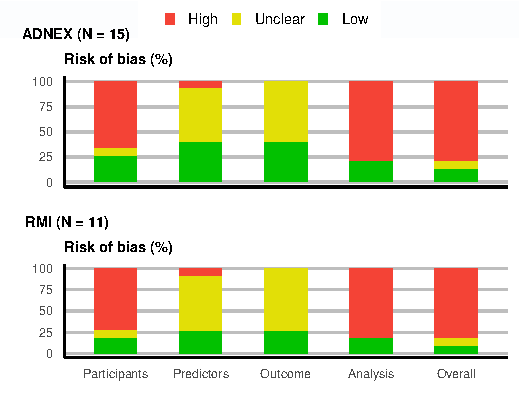
\includegraphics[width=0.8\textwidth]{figures/ADNEXvsRMI/F1.pdf}
\caption[PROBAST risk of bias for ADNEX and RMI validations]{Risk of bias by subdomain and overall for ADNEX and RMI validations using PROBAST. There are 15 validations of ADNEX and 11 validations of RMI.}
\label{fig:2:1}
\end{figure}

\subsection{Meta-analysis inclusions}
One study was excluded from the meta-analysis because it only presented results
stratified by the certainty of the ultrasound examiner when assessing the outcome
 \cite{szubertPerformanceSelectedModels2020}, and another study was excluded for not
reporting the cut-off used to calculate the sensitivity and specificity of \gls{ADNEX}
 \cite{ounPreoperativeRiskAssessment2023}. Therefore, nine studies were eligible for
meta-analysis
 \cite{vancalsterValidationModelsDiagnose2020,diazOvarianTumorsRisk2017a,tugPreoperativeDiscriminatingPerformance2020,behnamfarComparisonUltrasoundTumor2022,meysEstimatingRiskMalignancy2017,qianComparisonDiagnosticPerformances2021,sandalComparisionRiskMalignancy2018a,wangEvaluatingRiskMalignancy2023,borgesProspectiveExternalValidation2024}.
Four studies presented results for both \gls{ADNEX} versions (with and without CA125) and
five presented results only for \gls{ADNEX} with CA125. \gls{AUC} results were reported in all
studies except one \cite{sandalComparisionRiskMalignancy2018a}. However, one study
calculated \gls{AUC} after applying the threshold (i.e., based on a \gls{ROC} curve with one
single point) and thus was excluded from meta-analysis of \gls{AUC}
 \cite{wangEvaluatingRiskMalignancy2023}. Therefore, the meta-analysis of \gls{AUC} was
based on seven studies
 \cite{vancalsterValidationModelsDiagnose2020,diazOvarianTumorsRisk2017a,tugPreoperativeDiscriminatingPerformance2020,behnamfarComparisonUltrasoundTumor2022,meysEstimatingRiskMalignancy2017,qianComparisonDiagnosticPerformances2021,borgesProspectiveExternalValidation2024}.
Sensitivity and specificity at a 10\% risk of malignancy threshold for \gls{ADNEX} were
available (either in the publication or after contacting the authors) for all studies
except one (Table S4) \cite{behnamfarComparisonUltrasoundTumor2022}.

\subsection{Meta-analyses}
Results of the meta-analysis of \gls{AUC} are shown in Table~\ref{tab:2:2} and Figures S5 and S6. Seven studies included in
the meta-analysis compared the \gls{AUC} of \gls{ADNEX} (with CA125) with that of \gls{RMI} in
operated patients
 \cite{vancalsterValidationModelsDiagnose2020,diazOvarianTumorsRisk2017a,tugPreoperativeDiscriminatingPerformance2020,behnamfarComparisonUltrasoundTumor2022,meysEstimatingRiskMalignancy2017,qianComparisonDiagnosticPerformances2021,borgesProspectiveExternalValidation2024}.
The summary estimate for the \gls{AUC} in the four different meta-analyses varied between
0.92 and 0.94 for \gls{ADNEX}, and between 0.85 and 0.89 for \gls{RMI}. The summary estimate
for \gls{AUC} was higher for operated and conservatively managed patients combined (\gls{ADNEX}
0.93--0.94; \gls{RMI} 0.89) than for operated patients only (\gls{ADNEX} 0.92; \gls{RMI} 0.85--0.87).
\gls{RMI} had wider prediction intervals than \gls{ADNEX}. Figure~\ref{fig:2:2} shows the centre-specific or
study-specific comparison of \gls{ADNEX} with or without CA125 versus \gls{RMI} in operated
patients.

\begin{table}[ht!]
\centering
\tiny
\caption[Meta-analysis results for AUC]{Meta-analysis results for the area under the receiver operating characteristic curve (AUC).}
\label{tab:2:2}
% The first column is now an X column so tabularx can stretch it
\begin{tabularx}{\textwidth}{p{3cm} c c c c c c X}
\toprule
\textbf{Meta-analysis} & \textbf{Patients} & \textbf{Studies} & \textbf{Centres} & \textbf{Summary est.} & \textbf{95\% CI} & \textbf{95\% PI} & $\boldsymbol{\tau^2}$ \\
\midrule
\multicolumn{8}{l}{\textit{Target population: operated patients}} \\
\addlinespace
\multicolumn{8}{l}{\textbf{For ADNEX with CA125}} \\
\quad \quad ADNEX & 4668 & 7 & 26 & 0.92 & 0.90--0.94 & 0.82--0.99 & 0.30 \\
\quad \quad RMI   & 4668 & 7 & 26 & 0.85 & 0.81--0.89 & 0.64--0.98 & 0.44 \\
\addlinespace
\multicolumn{8}{l}{\textbf{For ADNEX without CA125}} \\
\quad \quad ADNEX & 3773 & 4 & 22 & 0.92 & 0.90--0.94 & 0.85--0.97 & 0.16 \\
\quad \quad RMI   & 3773 & 4 & 22 & 0.87 & 0.84--0.89 & 0.78--0.94 & 0.12 \\
\addlinespace
\multicolumn{8}{l}{\textit{Target population: operated and conservatively managed patients}} \\
\addlinespace
\multicolumn{8}{l}{\textbf{For ADNEX with CA125}} \\
\quad \quad ADNEX & 4905 & 1 & 17 & 0.93 & 0.91--0.96 & 0.85--0.99 & 0.27 \\
\quad \quad RMI   & 4905 & 1 & 17 & 0.89 & 0.86--0.92 & 0.77--0.97 & 0.22 \\
\addlinespace
\multicolumn{8}{l}{\textbf{For ADNEX without CA125}} \\
\quad \quad ADNEX & 4905 & 1 & 17 & 0.94 & 0.93--0.96 & 0.88--0.99 & 0.26 \\
\quad \quad RMI   & 4905 & 1 & 17 & 0.89 & 0.86--0.92 & 0.77--0.97 & 0.22 \\
\bottomrule
\addlinespace[0.5em]
% Replaced the 'l' column with a paragraph column that calculates the exact table width
\multicolumn{8}{p{\dimexpr\textwidth-2\tabcolsep\relax}}{ADNEX, Assessment of Different NEoplasias in the adneXa; CI, confidence interval; PI, prediction interval; RMI, risk of malignancy index.} \\
\end{tabularx}
\end{table}

\begin{figure}
\centering
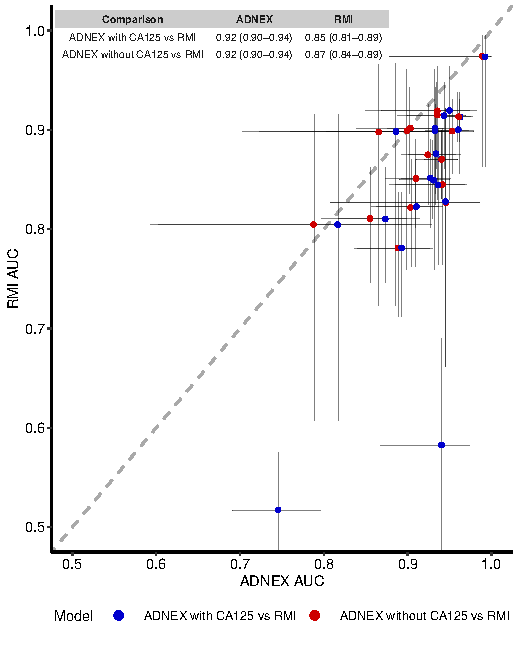
\includegraphics[width=0.8\textwidth]{figures/ADNEXvsRMI/F2.pdf}
\caption[Comparison of AUC of ADNEX and RMI per centre]{Comparison of the area under the receiver operating characteristic curve (AUC) of ADNEX (with and without CA125) and RMI per centre in the included studies for only operated patients. Vertical and horizontal lines present the CI of each centre's AUC. Dots below the diagonal line indicate higher AUC for ADNEX than for RMI. Dots above the diagonal line indicate higher AUC for RMI.}
\label{fig:2:2}
\end{figure}

The results of the meta-analysis for sensitivity and specificity are presented in
Table~\ref{tab:2:3} and Figures S7 and S8. Eight studies included in the meta-analysis compared the sensitivity and
specificity of \gls{ADNEX} (with CA125) with those of \gls{RMI} in surgically managed patients
 \cite{vancalsterValidationModelsDiagnose2020,diazOvarianTumorsRisk2017a,tugPreoperativeDiscriminatingPerformance2020,meysEstimatingRiskMalignancy2017,qianComparisonDiagnosticPerformances2021,sandalComparisionRiskMalignancy2018a,wangEvaluatingRiskMalignancy2023,borgesProspectiveExternalValidation2024}.
The summary estimate for sensitivity in the four different meta-analyses varied
between 0.92 and 0.94 for \gls{ADNEX} and was 0.61 for \gls{RMI} in all four analyses. The
summary estimate for specificity varied between 0.76 and 0.85 for \gls{ADNEX} and between
0.92 and 0.95 for \gls{RMI}. Specificity was higher for operated and conservatively managed
patients combined (ranging from 0.85 to 0.95) than for operated patients (ranging
from 0.76 to 0.93). Figure~\ref{fig:2:3} illustrates the centre-specific sensitivities and
specificities of \gls{ADNEX} and \gls{RMI} in patients managed with surgery in the space of a
receiver operating characteristic curve.

\begin{sidewaystable}
\centering
\scriptsize
\caption[Meta-analysis results for sensitivity and specificity]{Meta-analysis results for sensitivity and specificity at the 10\% risk of malignancy cut-off for ADNEX and at the 200 cut-off for RMI.}
\label{tab:2:3}
\begin{tabular}{llrc ccc ccc}
\toprule
& & & & \multicolumn{3}{c}{\textbf{Sensitivity}} & \multicolumn{3}{c}{\textbf{Specificity}} \\
\cmidrule(lr){5-7} \cmidrule(lr){8-10}
\textbf{Meta-analysis} & & \textbf{Patients} & \textbf{Studies (centres)} & \textbf{Summary est. (95\% CI)} & \textbf{95\% PI} & $\boldsymbol{\tau^2}$ & \textbf{Summary est. (95\% CI)} & \textbf{95\% PI} & $\boldsymbol{\tau^2}$ \\
\midrule
\multicolumn{10}{l}{\textbf{Target population: operated patients}} \\
\addlinespace
\multicolumn{10}{l}{\textbf{For ADNEX with CA125}} \\
& ADNEX & 5020 & 8 (26) & 0.93 (0.90--0.96) & 0.71--0.99 & 0.65 & 0.77 (0.71--0.81) & 0.46--0.92 & 0.38 \\
& RMI   & 5020 & 8 (26) & 0.61 (0.56--0.67) & 0.38--0.81 & 0.20 & 0.92 (0.89--0.94) & 0.75--0.98 & 0.39 \\
\addlinespace
\multicolumn{10}{l}{\textbf{For ADNEX without CA125}} \\
& ADNEX & 3773 & 4 (22) & 0.94 (0.90--0.96) & 0.66--0.99 & 0.81 & 0.76 (0.70--0.81) & 0.48--0.91 & 0.31 \\
& RMI   & 3773 & 4 (22) & 0.61 (0.56--0.67) & 0.40--0.79 & 0.16 & 0.93 (0.90--0.95) & 0.77--0.98 & 0.41 \\
\addlinespace
\multicolumn{10}{l}{\textbf{Target population: operated and conservatively managed patients}} \\
\addlinespace
\multicolumn{10}{l}{\textbf{For ADNEX with CA125}} \\
& ADNEX & 4905 & 1 (17) & 0.92 (0.87--0.96) & 0.55--0.99 & 0.99 & 0.85 (0.81--0.89) & 0.63--0.95 & 0.30 \\
& RMI   & 4905 & 1 (17) & 0.61 (0.54--0.67) & 0.38--0.80 & 0.17 & 0.95 (0.93--0.97) & 0.82--0.99 & 0.44 \\
\addlinespace
\multicolumn{10}{l}{\textbf{For ADNEX without CA125}} \\
& ADNEX & 4905 & 1 (17) & 0.92 (0.86--0.96) & 0.53--0.99 & 1.07 & 0.85 (0.80--0.88) & 0.62--0.95 & 0.29 \\
& RMI   & 4905 & 1 (17) & 0.61 (0.54--0.67) & 0.38--0.80 & 0.17 & 0.95 (0.93--0.97) & 0.82--0.99 & 0.44 \\
\bottomrule
\addlinespace[0.5em]
\multicolumn{10}{l}{ADNEX, Assessment of Different NEoplasias in the adneXa; CI, confidence interval; PI, prediction interval; RMI, risk of malignancy index; CrI, credible interval.}
\end{tabular}
\end{sidewaystable}

\begin{figure}
\centering
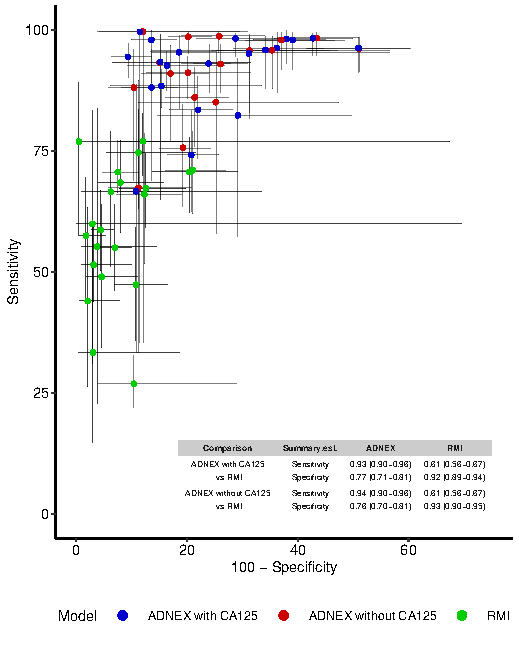
\includegraphics[width=0.8\textwidth]{figures/ADNEXvsRMI/F3.pdf}
\caption[Sensitivity and specificity of ADNEX and RMI in ROC space]{Sensitivity and specificity of ADNEX (10\% cut-off) and RMI (cut-off 200) in surgically managed patients illustrated in the space of a receiver operating characteristic curve. Each point represents the result of one study or centre and the lines represent the 95\% CI.}
\label{fig:2:3}
\end{figure}

The results for the meta-analysis of clinical utility are shown in Table~\ref{tab:2:4}. Based on
data from operated patients, the probability that the model would be clinically
useful in a new centre was 95\% to 96\% for \gls{ADNEX} and 13\% to 15\% for \gls{RMI}. Based on
data from both surgically and conservatively managed patients, the probability that
the model would be clinically useful in a new centre was 99\% for \gls{ADNEX} and 58\% for
\gls{RMI}.

\begin{sidewaystable}
\centering
\scriptsize
\caption[Meta-analysis results for clinical utility]{Meta-analysis for clinical utility of ADNEX and RMI.}
\label{tab:2:4}
\begin{tabular}{llrc cc cc c}
\toprule
& & & & \multicolumn{2}{c}{\textbf{Net benefit}} & \multicolumn{2}{c}{\textbf{Relative utility}} & \\
\cmidrule(lr){5-6} \cmidrule(lr){7-8}
\textbf{Meta-analysis} & & \textbf{Patients} & \textbf{Studies (centres)} & \textbf{Estimate (95\% CrI)} & \textbf{95\% PI} & \textbf{Estimate (95\% CrI)} & \textbf{95\% PI} & \textbf{P(useful)} \\
\midrule
\multicolumn{9}{l}{\textbf{Target population: operated patients}} \\
\addlinespace
\multicolumn{9}{l}{\textbf{For ADNEX with CA125}} \\
& ADNEX & 5020 & 8 (26) & 0.29 (0.21--0.37) & 0.05; 0.70 & 0.51 (0.40--0.61) & $-$0.11; 0.77 & 96\% \\
& RMI   & 5020 & 8 (26) & 0.19 (0.13--0.27) & 0.02; 0.60 & $-$0.80 ($-$1.3--$-$0.37) & $-$1.30; $-$0.37 & 15\% \\
\addlinespace
\multicolumn{9}{l}{\textbf{For ADNEX without CA125}} \\
& ADNEX & 3773 & 4 (22) & 0.30 (0.22--0.39) & 0.07; 0.67 & 0.48 (0.34--0.61) & $-$0.14; 0.78 & 95\% \\
& RMI   & 3773 & 4 (22) & 0.20 (0.13--0.28) & 0.02; 0.58 & $-$0.90 ($-$1.5--$-$0.45) & $-$3.97; 0.31 & 13\% \\
\addlinespace
\multicolumn{9}{l}{\textbf{Target population: operated and conservatively managed patients}} \\
\addlinespace
\multicolumn{9}{l}{\textbf{For ADNEX with CA125}} \\
& ADNEX & 4905 & 1 (17) & 0.17 (0.10--0.26) & 0.02; 0.61 & 0.69 (0.60--0.77) & 0.20; 0.85 & 99\% \\
& RMI   & 4905 & 1 (17) & 0.12 (0.06--0.19) & 0.01; 0.50 & 0.05 ($-$0.27--0.32) & $-$1.58; 0.53 & 58\% \\
\addlinespace
\multicolumn{9}{l}{\textbf{For ADNEX without CA125}} \\
& ADNEX & 4905 & 1 (17) & 0.17 (0.11--0.25) & 0.02; 0.59 & 0.68 (0.58--0.77) & 0.18; 0.85 & 99\% \\
& RMI   & 4905 & 1 (17) & 0.12 (0.06--0.19) & 0.01; 0.50 & 0.05 ($-$0.27--0.32) & $-$1.58; 0.53 & 58\% \\
\bottomrule
\addlinespace[0.5em]
\multicolumn{9}{l}{ADNEX, Assessment of Different NEoplasias in the adneXa; CI, confidence interval; PI, prediction interval; RMI, risk of malignancy index; CrI, credible interval.}
\end{tabular}
\end{sidewaystable}

\subsection{Certainty of evidence}
Based on the subdomains of the \gls{GRADE} assessment, we found that the risk of bias in
the studies included in this meta-analysis was a substantial limitation affecting the
certainty of our meta-analysis results. Only one study (representing 4905 patients or
59\% of the total number of patients included in this review) was not classified as
having a high risk of bias \cite{vancalsterValidationModelsDiagnose2020}. However,
the results of this low-risk of bias study and the current meta-analysis showed
consistent findings. Funnel plots for \gls{AUC} did not suggest publication bias (Figure S9).

\section{Discussion}

\subsection{Main findings}
This meta-analysis indicates that the ability of \gls{ADNEX}, with or without the
inclusion of CA125, outperforms \gls{RMI} in distinguishing benign from malignant adnexal
masses. It also suggests superior clinical utility of \gls{ADNEX} compared with \gls{RMI} when
applying the commonly recommended cut-offs (10\% malignancy risk for \gls{ADNEX} and \gls{RMI}
score 200) for determining which patients with an adnexal mass should be referred to
an oncology centre.

\subsection{Strengths and limitations}
Our meta-analysis is a comprehensive head-to-head comparison of external validations
of \gls{ADNEX} and \gls{RMI}. No previous study has conducted a systematic review and thorough
meta-analysis comparing these models head-to-head. A limitation is the high risk of
bias in all but one of the included studies and the poor reporting of \gls{TRIPOD} items.
Even though this is not a limitation of our meta-analysis, it affects our results.
Some of the reasons for high risk of bias, e.g., unknown or improper handling of
missing data (inappropriate exclusions), unclear information on blinding and small
sample size may have skewed the results of the included studies, and by extension,
the results of our meta-analysis. On the other hand, we found the summary estimates
for \gls{AUC}, sensitivity and specificity in the only study with low risk of bias
 \cite{vancalsterValidationModelsDiagnose2020} (a meta-analysis of data from 17
centres) to be very similar to those of the studies with high risk of bias. There was
considerable heterogeneity in model performance across studies. This is probably
explained by differences in study populations, settings or study designs. For
instance, very heterogeneous populations in terms of the model's predictors have
higher \glspl{AUC} \cite{vanleeuwenInstabilityAUROCClinical2025}. Rather than being a
limitation, heterogeneity could be seen as a good representation of how the models
perform under different conditions. Performance heterogeneity is commonly observed
for prediction models, even in studies that adhere to similar terms and definitions
and share a measurement protocol
 \cite{vancalsterValidationModelsDiagnose2020}. Due to the absence of reporting of
calibration performance in all but one of the included studies, we could not perform
meta-analysis of calibration performance, which is another limitation. It was also
not possible to meta-analyse net benefit over a range of risk thresholds.

\subsection{Interpretation}
There are published meta-analyses that compare the performance of different methods
to calculate the risk of malignancy in adnexal masses or to classify adnexal masses
as benign or malignant but that do not perform head-to-head comparisons
 \cite{kaijserPresurgicalDiagnosisAdnexal2014,meysSubjectiveAssessmentUltrasound2016}.
Meys and colleagues \cite{meysSubjectiveAssessmentUltrasound2016} reported a pooled
sensitivity of 0.75 (95\% \gls{CI} 0.72 to 0.79) and a pooled specificity of 0.92
(0.88--0.94) for \gls{RMI} at the 200 threshold based on 6970 masses from 14 studies.
Kaijser and colleagues \cite{kaijserPresurgicalDiagnosisAdnexal2014} found a pooled
sensitivity of 0.72 (0.67--0.76) and a pooled specificity of 0.92 (0.89--0.93)
based on 5626 patients from 23 studies, that is, their results were similar to those
of Meys et al \cite{meysSubjectiveAssessmentUltrasound2016}. These studies reported a
higher sensitivity than the current study. The most comprehensive meta-analysis of
the diagnostic performance of \gls{ADNEX} (47 studies, 17,007 adnexal masses) reports
meta-analysed summary estimates of \gls{AUC}, sensitivity, specificity and net benefit at
the 10\% risk of malignancy cut-off \cite{barrenadaADNEXRiskPrediction2024}. The
results are very similar to those in the current meta-analysis. An older multicentre
study (2403 patients; 18 centres) reported a higher clinical utility for \gls{ADNEX} than
for \gls{RMI} at cut-offs between 25 and 450. However, that study used a preliminary
version of the \gls{ADNEX} model \cite{wynantsClinicalUtilityRisk2017}.

In their article published in 1990, Jacobs et al discuss the choice of cut-off of
\gls{RMI} to decide which patients to refer to oncological care and state that if the
availability of such care is limited, then the cut-off can be set at 75 or 200
 \cite{jacobsRiskMalignancyIndex1990}. Many guidelines have adopted the 200 cut-off
 \cite{OvarianMassesPremenopausal2016a,AggstockscancerMedEpitelial2023,staer-jensenBenigneCysterOvarienea,HandteringAfOvariecyster2016,OvarianCystsPostmenopausal2016,sundarRiskpredictionModelsPostmenopausal2024}.
As shown in this meta-analysis, \gls{RMI} at 200 cut-off has low sensitivity (0.61) but
high specificity ($\geq$0.92). At this cut-off, a high proportion of stage one
ovarian malignancies, borderline tumours and secondary ovarian metastases will be
missed, but most advanced cancers will be detected
 \cite{vanholsbekeExternalValidationDiagnostic2012}. At the 10\% risk of malignancy
cut-off of \gls{ADNEX}, recommended in an international consensus statement
 \cite{timmermanESGOISUOGIOTA2021}, also borderline tumours and stage one primary
invasive ovarian malignancies will be detected and therefore referred to an oncology
centre, but so will many benign tumours (sensitivity in this
meta-analysis$\geq$0.92, specificity$\geq$0.76). This would seem to indicate that
lack of gynaecological oncological expertise is no longer a problem (in western
countries). This is supported by the recommendation of Sundar et al
 \cite{sundarRiskpredictionModelsPostmenopausal2024}. Sundar et al did a
head-to-head comparison of \gls{RMI} (cut-off 250) with \gls{ADNEX} in postmenopausal women
with symptoms suggestive of ovarian cancer in a real-world setting (ROCKeTS study).
They suggested, based on their results, that \gls{IOTA} \gls{ADNEX} at 10\% should be considered
the new standard-of-care diagnostic in ovarian cancer for postmenopausal patients
 \cite{sundarRiskpredictionModelsPostmenopausal2024}. This indicates that today high
sensitivity has priority over high specificity. The sensitivity of \gls{RMI} can be
increased by using a lower cut-off, e.g., 25 or 50. However, according to a
meta-analysis of data from 23 Italian centres, the clinical utility of \gls{ADNEX} is
superior to that of \gls{RMI} also at \gls{RMI} score 25
 \cite{moroExternalValidationUltrasoundbased2025}.

\section{Conclusion}

In conclusion, the results of our meta-analysis support that it is time to consider
replacing \gls{RMI} with \gls{ADNEX} in clinical guidelines, as suggested by Sundar and
colleagues \cite{sundarRiskpredictionModelsPostmenopausal2024}. The need for \gls{IOTA}
certification and adherence to a standardised examination technique and terminology
may present a challenge but should be seen as a necessary step in the evolution of
modern medical practice. Moreover, \gls{ADNEX} is integrated into ultrasound machines and
calculates the likelihood of four different types of malignant tumours. This makes it
a valuable tool for clinicians. \gls{ADNEX} works well also in the hands of ultrasound
examiners with limited ultrasound experience and when used in ``a real-world''
setting
 \cite{sundarRiskpredictionModelsPostmenopausal2024,moroExternalValidationUltrasoundbased2025}.

\section*{Acknowledgments}
We thank Thomas Vandendriessche, Chayenne Van Meel and Krizia Tuand, the biomedical
reference librarians of the KU Leuven Libraries (2Bergen, Learning Centre Désiré Collen, Leuven, Belgium) for their help in conducting the systematic literature
search. We gratefully acknowledge the authors of the external validations for
providing their valuable data.

\section*{Other information}
\subsection*{Funding}
This research was supported by the Research Foundation -- Flanders (FWO) under grant
G097322N with BVC and DT as supervisors. LW and BVC were supported by Internal Funds
KU Leuven (grant C24M/20/064). JYV was supported by the National Institute for
Health and Care Research (NIHR) Community Healthcare MedTech and In Vitro Diagnostics
Co-operative at Oxford Health NHS Foundation Trust (N/A). The views expressed are
those of the author(s) and not necessarily those of the NHS, the NIHR or the
Department of Health and Social Care. GSC is supported by Cancer Research UK
(programme grant: C49297/A27294). GSC is a National Institute for Health and Care
Research (NIHR) Senior Investigator. PD is supported by CRUK (project grant:
PRCPJT-Nov21\textbackslash100021). The funders had no involvement in study design;
collection, management, analysis and interpretation of data; or the decision to
submit for publication.

\subsection*{Conflicts of interest}
All authors have completed the ICMJE uniform disclosure form at
www.icmje.org/coi\_disclosure.pdf and declare: BVC, LV and DT are members of the
steering committee of the International Ovarian Tumour Analysis (\gls{IOTA}) consortium and
were involved in the development of the \gls{ADNEX} model. BVC and DT report consultancy
work done by KU Leuven to help implementing and testing the \gls{ADNEX} model in ultrasound
machines by Samsung Medison, GE Healthcare, Canon Medical Systems Europe and Shenzhen
Mindray Bio-medical Electronics, outside the submitted work. DT is co-founder of,
and BVC and DT have stock options in Gynaia Inc, a company providing teaching,
training and decision support tools such as the \gls{ADNEX} model for gynaecologists and
sonographers. All other authors have no competing interest to declare.

\subsection*{Availability of data and code}
Data and code to reproduce results and figures are available in a public, open access
repository (\url{https://osf.io/nt89z/}) \cite{barrenadaOSFADNEXVs2024}. All data
relevant to the study are included in the article or uploaded as supplementary
information. Some data were provided by the authors and were not public information;
therefore, this information was omitted from the public repository.

\subsection*{Contributors}
Contributions were based on the CRediT taxonomy. Conceptualisation: LB, BVC. Funding
acquisition: BVC, DT. Project administration: LB, AL. Supervision: BVC, LV, DT.
Methodology: LB, GSC, LW, JYJV, BVC. Resources: LB, AL. Investigation: LB, AL, LV,
BVC. Validation: LB, AL, PD, GSC, BVC. Data curation: LB, AL, JYJV, LV, BVC.
Software: LB, AL, LW, BVC. Formal analysis: LB, LW, BVC. Visualization: LB, AL.
Writing -- original draft: LB, AL, AK, DT, BVC. Writing -- review \& editing: all
authors. BVC is the guarantor and takes full responsibility for the overall content
of the manuscript. All authors have read, share final responsibility for the decision
to submit for publication and agree to be accountable for all aspects of the work.

\subsection*{Ethics approval}
Not applicable.
